\section{Methodology}

\subsection{Background and Problem Formulation}\label{subsec:problem_formulation}
We consider a setup containing $M$ environments. For each environment $m \in \cS = \{1,\dots,M\}$, we consider the multipath propagation between transmitters (tx) $b \in \cB_m$ and receivers (rx) $u \in \cU_m$ distributed throughout the environment.  For each tx-rx pair $(m,b,u)$, we get the tx and rx positions $\vect{x}_{\mathrm{tx}}^{(m,b)}, \vect{x}_{\mathrm{rx}}^{(m,u)}  \in \R^3$, environment features $\vect{x}_{m} \in \R^{d_{env}}$,  multipath sequence $\cP_{m,b,u}$, and the corresponding channel tensor $\vect{H}_{m,b,u}$.  We show an example of such an environment in Figure \ref{fig:env_kmeans_overview}{a}.  A multipath sequence 
 with $L_{m,b,u}$ number of mulitpath is defined in Equation \ref{eqn:multpathset}. 
% $\cP_{m,b,u} \in \R^{L_{m,b,u} \times 8}$
\begin{equation}
\cP_{m,b,u} = \big(\pi^{(m,b,u)}_1,\ldots,\pi^{(m,b,u)}_{L_{m,b,u}}\big),
\label{eqn:multpathset}
\end{equation}

\begin{equation}
\pi^{(m,b,u)}_\ell = \Big(\rho_\ell, \phi_\ell, \tau_\ell, \theta^{\mathrm{aoa}}_{\ell,\mathrm{az}}, \theta^{\mathrm{aoa}}_{\ell,\mathrm{el}}, \theta^{\mathrm{aod}}_{\ell,\mathrm{az}}, \theta^{\mathrm{aod}}_{\ell,\mathrm{el}}, \vect{z}_\ell\Big).
\label{eq:path_descriptor}
\end{equation}

Each multipath $\pi^{(m,b,u)}_\ell$ component is defined in \ref{eq:path_descriptor}, where $\rho_\ell$ is the path power, $\phi_\ell$ is the phase, $\tau_\ell$ is the propagation delay, $\theta^{\mathrm{aoa}}_{\ell,\mathrm{az}}$ and $\theta^{\mathrm{aoa}}_{\ell,\mathrm{el}}$ are the azimuth and elevation angles of arrival, $\theta^{\mathrm{aod}}_{\ell,\mathrm{az}}$ and $\theta^{\mathrm{aod}}_{\ell,\mathrm{el}}$ are the corresponding angles of departure, and $\vect{z}_\ell$ is an interaction type experienced by the path. The interaction type $\vect{z}_\ell \in  \{0,1\}^4 $ is a multihot vector showing if the path experiences Reflection, Diffraction, Scattering or LoS.

\begin{figure*}[t]
    \centering
    \begin{minipage}[t]{0.49\textwidth}
        \centering
        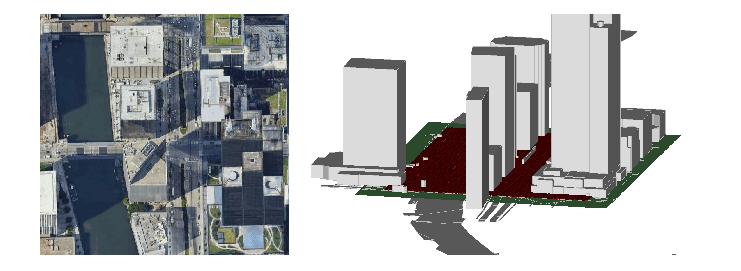
\includegraphics[height=3.0cm, width=\linewidth]{figures/user_grid_env.pdf}
        
        \vspace{2pt}
        \small \textbf{a)} Physical Environment and 3D user grid
    \end{minipage}
    \hfill
    \begin{minipage}[t]{0.49\textwidth}
        \centering
        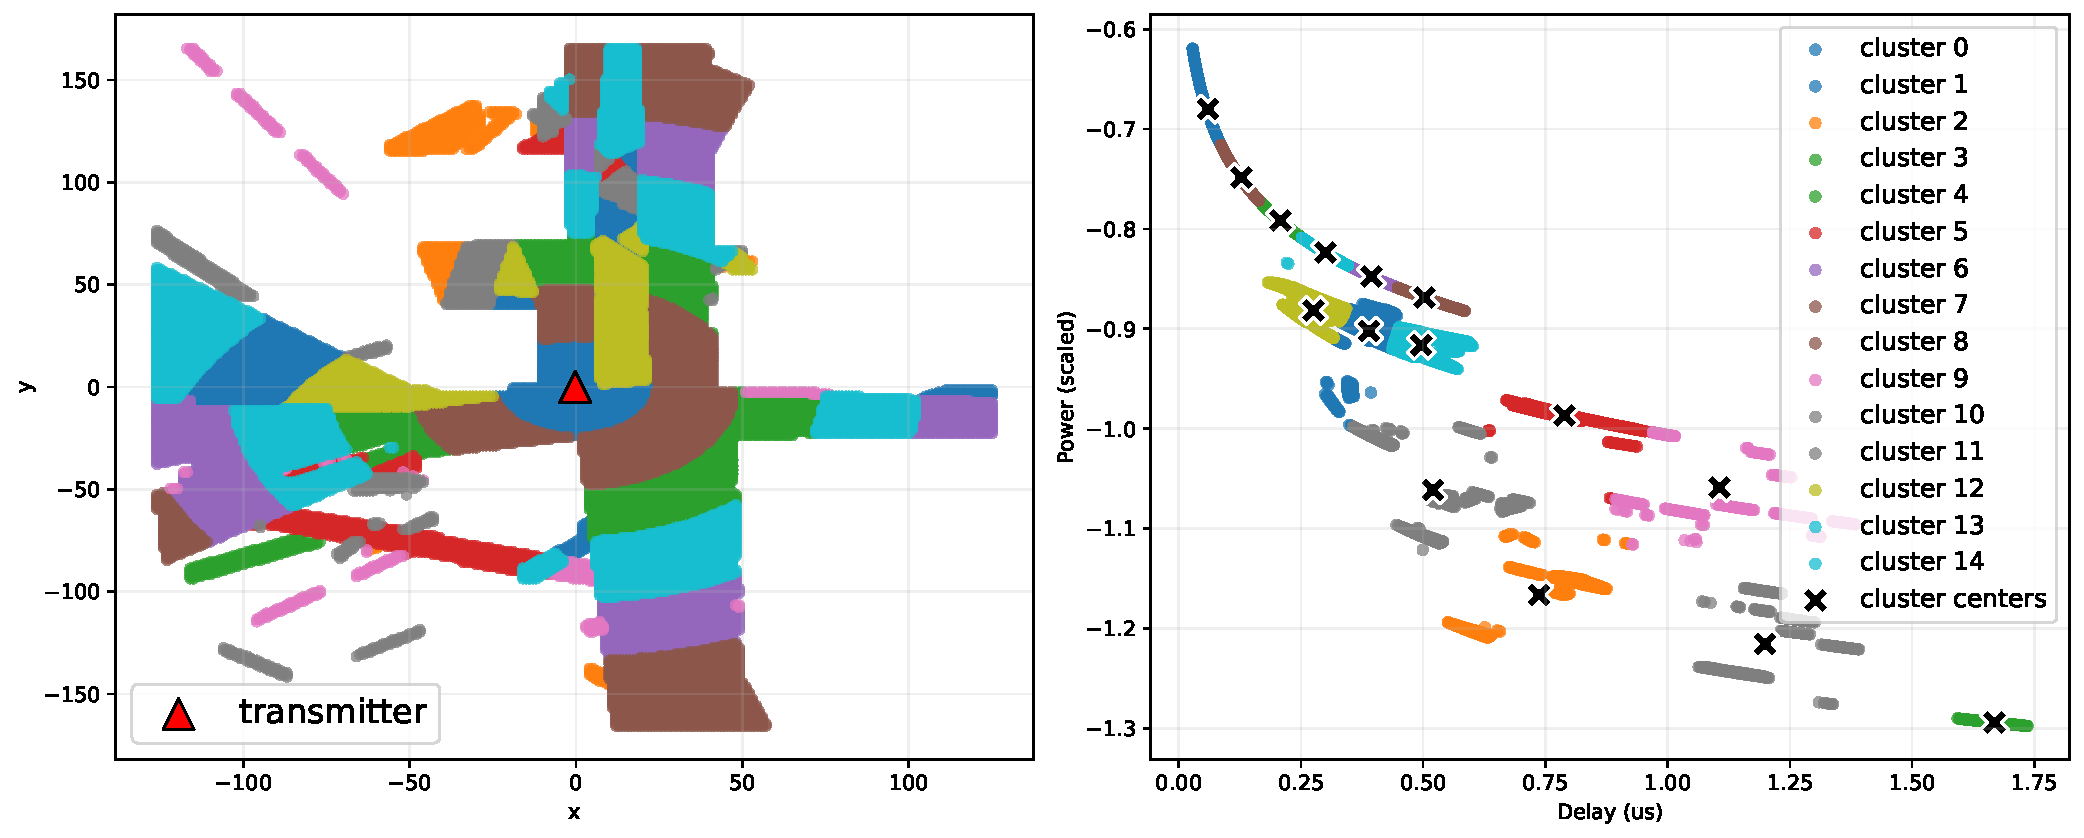
\includegraphics[height=3.0cm, width=\linewidth]{figures/first_timestep_user_kmeans.pdf}
        
        \vspace{2pt}
        \small \textbf{b)} Physical environment
    \end{minipage}
    \hfill
    \caption{
    \textbf{a)} The physical environment  and the corresponding 3D model.
    \textbf{b)} User clusters obtained from KMeans on first-path delay and power, showing that users organize into spatially coherent groups under a fixed transmitter.
    }
    \label{fig:env_kmeans_overview}
\end{figure*}

For a tx-rx pair with some features from its environment, we formulate the autoregressive modelling objective in Equation \ref{eq:next_path} to predict the arrival of the next multipath given the previous multipaths. This autoregressive formulation lends itself naturally to physical propagation because of how it closely aligns with the decay of power over subsequent paths or how paths arrive sequentially with increasing delays.

\begin{equation}
p_{\theta}(\cP_{m,n}\mid e_m)
=
\prod_{t=1}^{L_{m,n}+1}
p_{\theta}(\pi^{(m,b,u)}_t  \mid \pi^{(m,b,u)}_{<t},\vect{x}_{\mathrm{rx}}^{(m,u)}, \vect{x}_{\mathrm{tx}}^{(m,b)}, \vect{x}_{m} ).
\label{eq:next_path}
\end{equation}

This formulation leads us to \textit{solving an autoregressive variable sequence length regression problem}. This is different from the standard autoregressive formulation in language modelling for two reasons. First, in language modelling, tokens are derived from the text, yielding a vocabulary, and the model solves a \textit{variable sequence length autoregressive classification problem} over the vocabulary. Secondly, in language modelling, start and stop tokens are added to the vocabulary to initiate and terminate generation, which is not straightforward to do in a regression setup. To solve this, we first convert the path set into a deterministic ordered sequence by sorting the paths by descending power $\rho_{m,n,1} \ge \rho_{m,n,2} \ge \cdots \ge \rho_{m,n,L_{m,n}}$. The other option is to sort based on delay, because, as shown in Figure \ref{fig:env_kmeans_overview}{b}, we do not have a perfect inverse-linear relationship between received power and delay. However, we do not find any significant performance differences between the two setups. We create a start token of a vector of max power, no delays and zero angles $\pi^{(m,b,u)}_0 ={\textbf{0}}$ to initiate generation. At each timestep, the model simulatenously predicts the path parameters defined in Equation \ref{eq:path_descriptor}.  To terminate generation, rather than define a target end-of-sentence path, which could hurt the performance in a regression setup, we explicitly predict the number of paths between the transmitter and receiver and use that to terminate. Analogously to how Retrieval Augmented Generation (RAG) has helped to augment language prompts with relevant context, we propose an \textit{Environmental RAG framework }in section \ref{subsec:env_rag} on how to extract the relevant environmental features $\vect{x}_{m}$ relevant to the tx-rx pair. 
\subsection{PathFormer Backbone Model}
We propose to solve the problem formulated in \ref{eq:next_path} with our Pathformer Model. The Pathformer model uses an encoder-decoder transformer architecture similar to Vision Language Models\cite{li2023trocr,alayrac2022flamingo}, with the encoder and decoder capturing information from different modalities.  The encoder produces representations capturing the relationship between tx-rx and the physical environment. To encourage the encoder to produce environmentally grounded representations and also to solve the variable sequence length introduced in Section \ref{subsec:problem_formulation}, we supervise the encoder's representation to be predictive of the number of multipaths between the tx-rx. The decoder then captures how the current path relates to previous paths conditioned on the environment encoder's representations. Therefore, the encoder works in the physical environment modality, and the decoder primarily works in the EM multipath modality. This process in the pathformer to produce the hidden state at generation step $t$ is captured in Equation \ref{eq:backbone}. 
\begin{figure}
    \centering
    \fbox{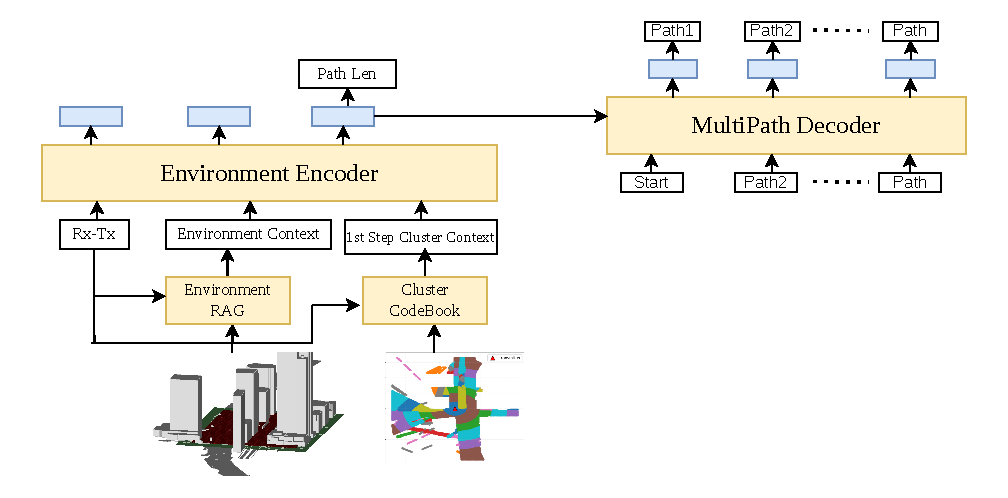
\includegraphics[width=\linewidth]{figures/PathFormer-Page-7.drawio.pdf}}
    \caption{
    Overview of the proposed corridor-aware PathFormer. The model augments the tx-rx prompt with Environmental RAG features and a first-path KMeans codebook, then autoregressively predicts the multipath sequence with a residual correction for the dominant first path.
    }
    \label{fig:pathformer_corridor}
\end{figure}

\begin{equation}
\vect{E}_{env}
=
\mathrm{Encoder}_{\theta}( [x_m, x_{tx}, x_{rx}] )
\label{eq:backbone}
\end{equation}

\begin{equation}
\hat{L}_{m,b,u}
=
f_{\mathrm{len}}(\vect{E}_{\mathrm{env}}),
\label{eq:pathformer_length_head}
\end{equation}

\begin{equation}
\vect{h}_t
=
\mathrm{Decoder}_{\theta}
\Big(
[\vect{E}_{env};\,E_{\mathrm{tok}}(o_{<t}) + \vect{p}_{<t}]
\Big),
\label{eq:backbone}
\end{equation}
From $\vect{h}_t$, the model predicts the next path token $\widehat{\vect{y}}_t$ including the interactions experienced  $\hat{\vect{z}}_t \in [0,1]^4$ using Equations \ref{eq:pathformer_reg_head} and \ref{eq:pathformer_interaction_head}. Each element in $\hat{\vect{z}}_t$ is the corresponding probabilities for the interaction labels. This is because a path may simultaneously experience multiple interaction types (e.g. reflection and refraction), predicting $\vect{z}_t$ is a \emph{multilabel classification problem} with its loss defined in Equation \ref{eq:interaction_loss}.
\begin{equation}
\widehat{\vect{y}}_t =
\Big(
\hat{\tau}_t,\hat{\rho}_t,
\widehat{\sin\phi_t},\widehat{\cos\phi_t},
\widehat{\sin\theta^{\mathrm{aoa}}_{t,\mathrm{az}}},\widehat{\cos\theta^{\mathrm{aod}}_{t,\mathrm{az}}},
\widehat{\sin\theta^{\mathrm{aoa}}_{t,\mathrm{el}}},\widehat{\cos\theta^{\mathrm{aod}}_{t,\mathrm{el}}}
\Big)
=
W_{\mathrm{reg}}\vect{h}_t + \vect{b}_{\mathrm{reg}},
\label{eq:pathformer_reg_head}
\end{equation}

\begin{equation}
\vect{s}_t
=
W_{\mathrm{int}}\vect{h}_t + \vect{b}_{\mathrm{int}},
\qquad
\hat{\vect{z}}_t = \sigma(\vect{s}_t),
\label{eq:pathformer_interaction_head}
\end{equation}
For a path with length $L_{m,b,u}$ We compute an L2 loss for the other parameters and the path length in (Equations \ref{eq:path_l2_loss_transformed} and \ref{eq:path_length_loss}). We define total loss as a weighted combination of these three objectives in Equation \ref{eq:total_loss}.

\begin{equation}
\mathcal{L}_{\mathrm{path}}
=
\frac{1}{L_{m,b,u}}
\sum_{t}
\left\|
\hat{\vect{y}}_t-\vect{y}_t
\right\|_2^2,
\label{eq:path_l2_loss_transformed}
\end{equation}

\begin{equation}
\mathcal{L}_{\mathrm{len}}
=
\left(
\hat{L}_{m,b,u}-L_{m,b,u}
\right)^2,
\label{eq:path_length_loss}
\end{equation}


\begin{equation}
\mathcal{L}_{\mathrm{int}}
=
\frac{1}{L_{m,b,u}}
\sum_{t}\sum_{k=1}^{4}
\left[
-z_{t,k}\log \sigma(s_{t,k})
-(1-z_{t,k})\log\big(1-\sigma(s_{t,k})\big)
\right],
\label{eq:interaction_loss}
\end{equation}

\begin{equation}
\mathcal{L}
=
\mathcal{L}_{\mathrm{path}}
+
\lambda_{\mathrm{int}}\mathcal{L}_{\mathrm{int}}
+
\lambda_{len}\mathcal{L}_{len}
\label{eq:total_loss}
\end{equation}

\subsection{Environmental Retrieval Augmented Generation}
\label{subsec:env_rag}

During propagation, multipaths interact with a variety and density of objects in the environment. Environments can vary starkly, with sparser buildings in less populated areas to more dense objects and users in urban settings. We, however, require our model to be able to reason about relevant objects in all types of environments in an efficient manner.
The naive approach of passing a single global environment descriptor $\vect{x}_m$ may be too coarse, noisy and inefficient for path prediction for disambiguating users across different varying environments. The paths for a tx-rx pair are determined not only by which environment the pair belongs to, but more specifically by \emph{which objects are locally close to the receiver and which objects lie along the tx-rx propagation corridor}. This motivates our \emph{Environmental Retrieval RAG} framework, which retrieves tx-rx-specific geometric context from the scene and conditions the Pathformer on this retrieved representation. We consider an environment $m$, with tx-rx pair located at $\vect{p}^{(m,b)}_{\mathrm{tx}}, \vect{p}^{(m,u)}_{\mathrm{rx}} \in \mathbb{R}^2$, with   $\mathcal{O}_m=\{o^{(m)}_1,\dots,o^{(m)}_{J_m}\}$
denoting the set of physical objects in the scene. Each object $o^{(m)}_j$ is associated with geometric attributes such as planar centroid $\vect{p}^{(m)}_j\in\mathbb{R}^2$, height $h^{(m)}_j$, footprint area $a^{(m)}_j$, and material properties.

\paragraph{Local dense retrieval.}
For a query point $\vect{q}\in\mathbb{R}^2$ and radius $d_{\max}$, we define the local object candidate set in Equation \ref{eq:candidate_set} and retain the $K$ nearest objects \ref{eq:local_retrieval}.
\begin{equation}
\mathcal{O}_{m}(\vect{q}, d_{\max})
=
\left\{
o_j \in \mathcal{O}_m :
\left\|
\vect{p}^{(m)}_j-\vect{q}
\right\|_2 \le d_{\max}
\right\},
\label{eq:candidate_set}
\end{equation}

\begin{equation}
\mathcal{N}_{K}(\vect{q}, d_{\max})
=
\operatorname{TopK}_{o_j \in \mathcal{O}_{m}(\vect{q}, d_{\max})}
\left\|
\vect{p}^{(m)}_j-\vect{q}
\right\|_2 .
\label{eq:local_retrieval}
\end{equation}
We apply this retrieval at both $\vect{q}=\vect{p}^{(m,u)}_{\mathrm{rx}}$ and $\vect{q}=\vect{p}^{(m,b)}_{\mathrm{tx}}$. For each retrieved object, we keep a dense description consisting of distance, height, footprint area, and material properties. 



\paragraph{Corridor dense retrieval.}
To capture objects that are not close to either endpoint but still lie near the propagation route, we define a tx-rx corridor. For each object $o_j$ with its centroid at $p_{j}$, we project it onto the tx-rx line using Equation \ref{eq:corridor_segment} and then compute the distance of the object to that point on the tx-rx line segment in Equation \ref{eq:corridor_distance}. Finally, we then retrieve Top-k close objects in a similar manner to Equation \ref{eq:local_retrieval}.
% \begin{equation}
% \mathcal{C}_{m,b,u}(j)
% =
% \vect{p}^{(m,b)}_{\mathrm{tx}}
% +
% \alpha_j
% \big(\vect{p}^{(m,u)}_{\mathrm{rx}}-\vect{p}^{(m,b)}_{\mathrm{tx}}\big),
% \label{eq:corridor_segment}
% \end{equation}
% where
% \begin{equation}
% \alpha_j
% =
% \frac{
% (\vect{p}^{(m)}_j-\vect{p}^{(m,b)}_{\mathrm{tx}})^\top
% (\vect{p}^{(m,u)}_{\mathrm{rx}}-\vect{p}^{(m,b)}_{\mathrm{tx}})
% }{
% \left\|
% \vect{p}^{(m,u)}_{\mathrm{rx}}-\vect{p}^{(m,b)}_{\mathrm{tx}}
% \right\|_2^2
% }.
% \label{eq:projection_coeff}
% \end{equation}

\begin{equation}
\mathcal{C}_{m,b,u}(j)
=
\vect{p}^{(m,b)}_{\mathrm{tx}}
+
\text{proj}_{\mathbf{\vect{p}^{(m,u)}_{\mathrm{rx}}-\vect{p}^{(m,b)}_{\mathrm{tx}}}} (\vect{p}^{(m)}_j-\vect{p}^{(m,b)}_{\mathrm{tx}} )
\label{eq:corridor_segment}
\end{equation}

\begin{equation}
d^{\mathrm{cor}}_j
=
\left\|
\vect{p}^{(m)}_j-\mathcal{C}_{m,b,u}(j)
\right\|_2.
\label{eq:corridor_distance}
\end{equation}

% In practice, we clip $\alpha_j$ to $[0,1]$ so that $\mathcal{C}_{m,b,u}(j)$ lies on the finite transmitter--receiver segment rather than on its infinite line extension. We then retain the $K$ closest objects within corridor radius $d_{\max}$:
% \begin{equation}
% \mathcal{N}^{\mathrm{cor}}_{K}(d_{\max})
% =
% \operatorname{TopK}_{o_j \in \mathcal{O}_m:\, d^{\mathrm{cor}}_j \le d_{\max}}
% d^{\mathrm{cor}}_j .
% \label{eq:corridor_retrieval}
% \end{equation}


\paragraph{Sparse multi-scale summaries.}
The dense top-$K$ retrieval captures the most relevant individual objects but not the broader spatial distribution of clutter. Moreover, we need to capture to capture some summarised information about objects within $d_{max}$ but not captured in the top-$K$.  We therefore add sparse summaries computed over increasing radii $\{d_1,\dots,d_R\}$.  Around both the transmitter and receiver, we compute object counts and maximum object heights within each radius. Similarly, around the tx-rx corridor, we partition the tx-rx segment into $B$ bins and, within corridor radius $d_{\max}$, compute per-bin summaries of object count and maximum height. These sparse features provide a coarse multi-scale description of environmental density and obstruction patterns. We concatenate the local, dense, and sparse summaries around to have our full retrieval context.
\begin{equation}
\vect{r}_{m,b,u}
=
\psi\!\Big(
\mathcal{N}_{K}(\vect{p}^{(m,u)}_{\mathrm{rx}}, d_{\max}),
\mathcal{N}_{K}(\vect{p}^{(m,b)}_{\mathrm{tx}}, d_{\max}),
\mathcal{N}^{\mathrm{cor}}_{K}(d_{\max})
\Big),
\label{eq:retrieval_vector}
\end{equation}
where $\psi(\cdot)$ concatenates: (i) dense features for the top-$K$ local objects around the receiver and transmitter, (ii) dense features for the top-$K$ objects nearest to the transmitter--receiver corridor, and (iii) sparse multi-scale summaries over local radii and corridor bins. This representation is both efficient and pair-specific: the dense component preserves the most relevant object-level information, while the sparse component captures broader environmental structure.


\paragraph{First-Path Cluster CodeBook.}
Because the path sequence is sorted by descending power, the first path often corresponds to the dominant propagation mode. Empirically, this first path exhibits strong spatial regularity: nearby users served by the same transmitter often share similar first-path delay and power. We exploit this structure by learning a transmitter-specific KMeans prior over the first-path target
\begin{equation}
\vect{y}^{(1)}_{m,b,u}
=
\begin{bmatrix}
\tau_1^{(m,b,u)}\\
\rho_1^{(m,b,u)}
\end{bmatrix}.
\label{eq:first_path_target}
\end{equation}

For each transmitter $b$ in environment $m$, we fit KMeans on the training set:
\begin{equation}
\{\vect{c}^{(m,b)}_k\}_{k=1}^{K}
=
\mathrm{KMeans}\!\left(
\{\vect{y}^{(1)}_{m,b,u}:u\in\mathcal{U}^{\mathrm{train}}_m\}
\right),
\label{eq:kmeans_centers}
\end{equation}
where $\vect{c}^{(m,b)}_k\in\mathbb{R}^2$ is the $k$-th cluster centroid. We also compute the within-cluster dispersion
\begin{equation}
\vect{\sigma}^{(m,b)}_k
=
\mathrm{Std}\!\left(
\{\vect{y}^{(1)}_{m,b,u}: z^{(m,b,u)}=k\}
\right),
\label{eq:kmeans_std}
\end{equation}
where $z^{(m,b,u)}$ is the cluster assignment.

At test time, a receiver is assigned a first-path prior through nearest-neighbor transfer within the same transmitter:
\begin{equation}
u^\star
=
\arg\min_{u' \in \mathcal{U}^{\mathrm{train}}_m(b)}
\left\|
\vect{x}^{(m,u)}_{\mathrm{rx}}
-
\vect{x}^{(m,u')}_{\mathrm{rx}}
\right\|_2^2,
\label{eq:nn_assignment}
\end{equation}
and the corresponding cluster prior is
\begin{equation}
\vect{c}_{m,b,u}=\vect{c}^{(m,b)}_{z^{(m,b,u^\star)}},
\qquad
\vect{\sigma}_{m,b,u}=\vect{\sigma}^{(m,b)}_{z^{(m,b,u^\star)}}.
\label{eq:assigned_cluster_prior}
\end{equation}

\paragraph{Residual First-Path Prediction.}
We use the KMeans centroid as a strong initialization for the first path, and train the model to predict only the residual correction:
\begin{equation}
\widehat{\vect{y}}^{(1)}_{m,b,u}
=
\vect{c}_{m,b,u}
+
f_{\mathrm{res}}
\Big(
\vect{h}_1,\,
\vect{c}_{m,b,u},\,
\vect{\sigma}_{m,b,u},\
\vect{r}_{m,b,u}
\Big),
\label{eq:first_path_residual}
\end{equation}
where $\vect{h}_1$ is the decoder hidden state at the first generation step. This design is important: the KMeans prior captures a strong spatial mode for the dominant path, while the residual term allows the network to adapt that prior using the retrieved environmental geometry. In other words, KMeans provides a robust default hypothesis, and Environmental RAG provides the scene evidence needed to refine it. For subsequent paths $t\geq 2$, the model reverts to the standard autoregressive prediction defined by the PathFormer decoder. Thus, the full framework combines:
(i) retrieval of tx-rx pair-specific environmental context,
(ii) a cluster codebook prior for the dominant path, and
(iii) autoregressive sequence modeling for the remaining multipath components.

% \paragraph{Intuition.}
% The proposed Environmental RAG framework addresses two limitations of using only a coarse environment embedding. First, local receiver-side features alone cannot explain dominant blockers or reflectors that lie far from the receiver but directly along the propagation route. Second, learning the first path entirely from scratch forces the network to rediscover a strong low-dimensional spatial prior that can be estimated much more reliably with a simple clustering model. By combining corridor-aware retrieval with a KMeans-based first-path prior, the model receives both \emph{geometric scene evidence} and a \emph{strong dominant-path initialization}, leading to more stable and physically grounded predictions.


\subsection{Multi-Environment Pretraining and Finetuning}\label{sec:pretrain_finetune}
% Since multipath propagation exhibits both environment-specific structure and cross-environment regularities, we adopt a two-stage training strategy. First, we pretrain PathFormer jointly across multiple environments so that it learns general sequential regularities of multipath generation. We then finetune the pretrained backbone on a target environment, where the transmitter and receiver geometry is provided explicitly. During multi-environment pretraining (Equation \ref{eq:pretraining}), we mask the transmitter and receiver locations so that the model cannot rely on user-specific geometry and must instead capture environment-level and sequence-level propagation patterns.
% \begin{equation}
% \vect{E}_{env}^{\mathrm{pre}}
% =
% \mathrm{Encoder}_{\theta}\big([\,\vect{x}_m,\vect{0}_{tx},\vect{0}_{rx}\,]\big).
% \label{eq:pretraining}
% \end{equation}
% The foundation model here is optimised over samples drawn from all training environments on the objective in Equation \ref{eq:total_loss}. In this way, the model learns a user-agnostic foundation prior over multipath sequences. After pretraining, the model is adapted to a target environment by restoring the transmitter and receiver locations:
% \begin{equation}
% \vect{E}_{env}^{\mathrm{ft}}
% =
% \mathrm{Encoder}_{\theta}\big([\,\vect{x}_m,\vect{x}_{tx},\vect{x}_{rx}\,]\big).
% \label{eq:finetuning}
% \end{equation}
% Starting from the pretrained parameters $\theta_{\mathrm{pre}}$, we finetune the model on environment-specific samples to obtain
% \begin{equation}
% \theta_{\mathrm{ft}}
% =
% \arg\min_{\theta}
% \mathbb{E}_{(m,b,u)\sim \mathcal{D}_{\mathrm{target}}}
% \left[
% \mathcal{L}_{\mathrm{path}}
% +
% \lambda_{\mathrm{len}}\mathcal{L}_{\mathrm{len}}
% +
% \lambda_{\mathrm{int}}\mathcal{L}_{\mathrm{int}}
% \right].
% \label{eq:finetune_loss}
% \end{equation}
% This stage adapts the general sequential prior learned during pretraining to the geometry and propagation dynamics of the target environment.

\subsection{Downstream Task Reuse}\label{sec:down}
We describe how the foundation model can be used for the downstream tasks, both in \emph{zero-shot style and adapter finetuning}. We consider the tasks of \textit{beam prediction, user-localisation, and channel estimation}. 
For the adapter fine-tuning, we freeze the backbone Pathformer model and finetune some MLP heads for some downstream tasks. This leverages the generalised representations from the pathformer backbone and allows for efficient finetuning of few parameters from the added MLP heads. We apply a pool function (e.g. mean, first) to the hidden representation produced during autoregressive rollout as shown in Equation \ref{eq:pool}. 

\begin{equation}
\bar{\vect{h}}_{m,n} = \Pool\big(\vect{h}_1,\ldots,\vect{h}_{\hat{L}_{m,n}}\big)
\label{eq:pool}
\end{equation}


\paragraph{Channel reconstruction.}
The predicted path sequence can be rendered back into a channel estimate using the same physical model,
\begin{equation}
\hat{\vect{H}}_{m,n}[k]
=
\sum_{t=1}^{\hat{L}_{m,n}}
\hat{\alpha}_{m,n,t}
\exp\!\left(-j2\pi f_k\hat{\tau}_{m,n,t}\right)
\vect{a}_{\mathrm{rx}}\!\left(\hat{\theta}^{\mathrm{aoa}}_{m,n,t,\mathrm{az}},\hat{\theta}^{\mathrm{aoa}}_{m,n,t,\mathrm{el}}\right).
\label{eq:channel_reconstruction}
\end{equation}
The resulting channel can be evaluated using
\begin{equation}
\NMSE
=
\frac{\sum_{k \in \cK}\|\hat{\vect{H}}[k]-\vect{H}[k]\|_F^2}
{\sum_{k \in \cK}\|\vect{H}[k]\|_F^2}.
\label{eq:nmse}
\end{equation}

\paragraph{Beam prediction}
Given a beam codebook $\mathcal{W}=\{\vect{w}_1,\ldots,\vect{w}_{|\mathcal{W}|}\}$, beam selection from the reconstructed channel can be written as
\begin{equation}
\hat{b}_{m,n}
=
\arg\max_{q \in \{1,\ldots,|\mathcal{W}|\}}
\sum_{k \in \cK}
\left\|\vect{w}_q^{H}\hat{\vect{H}}_{m,n}[k]\right\|_2^2.
\label{eq:beam_selection}
\end{equation}
A lightweight classifier head on $\bar{\vect{h}}_{m,n}$ can also be used if desired.

\paragraph{User Localization.}
For user localization, a regression head is attached to the pooled hidden state,
\begin{equation}
\hat{\vect{x}}^{\mathrm{rx}}_{m,n} = f_{\mathrm{loc}}(\bar{\vect{h}}_{m,n}).
\label{eq:localization}
\end{equation}
This evaluates whether the pretrained backbone captures information that is useful not only for forward channel synthesis but also for inverse geometric inference.